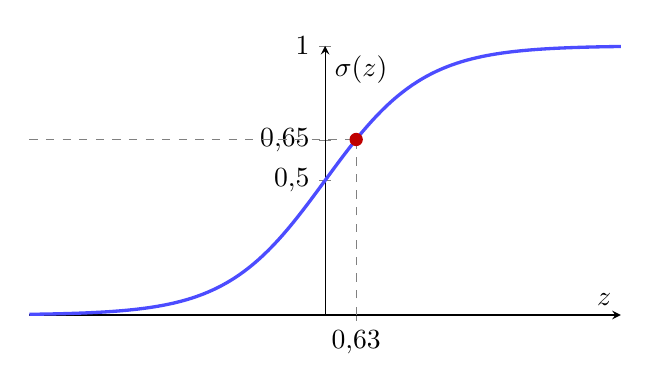
\begin{tikzpicture}
    \begin{axis}[
        width=0.75\textwidth,
        height=5cm,
        xmin=-6, xmax=6,
        ymin=0, ymax=1,
        axis lines=middle,
        xlabel={$z$},
        ylabel={$\sigma(z)$},
        xtick={0,0.63},
        xticklabels={$0$,$0{,}63$},
        ytick={0,0.5,0.65,1},
        yticklabels={$0$,$0{,}5$,$0{,}65$,$1$},
        clip=false
    ]
        \addplot[
            very thick,
            blue!70,
            domain=-6:6,
            samples=120
        ] {1/(1+exp(-x))};

        \addplot[dashed, gray] coordinates {
            (0.63,0) (0.63,0.652)
        };

        \addplot[dashed, gray] coordinates {
            (-6,0.652) (0.63,0.652)
        };

        \addplot[
            only marks,
            mark=*,
            mark size=2.2pt,
            red!75!black
        ] coordinates {
            (0.63,0.652)
        };
    \end{axis}
\end{tikzpicture}
